\section{Experiments and Current Status}\label{sec:experiments}

So far, the functional basis of \method has been implemented in its web version.
The most relevant partial result is the consolidation of a complete flow, still under validation, that goes from the creation of a geographic project to the generation of a preliminary sewer network processed by graph algorithms.
The current version already allows users to create and list projects, open the editor, visualize streets and nodes, edit the graph, run the pipeline, save the processed network, and reload the persisted state.
Figure~\ref{fig:before-after-processing} shows a local example of this transformation, comparing the enriched editable graph before processing with the directed network produced after the pipeline.

\begin{figure}[H]
\centering
\begin{minipage}{.49\linewidth}
\centering

\includegraphics[width=\linewidth]{images/small-case-before-processing.png}
\end{minipage}
\hfill
\begin{minipage}{.49\linewidth}
\centering
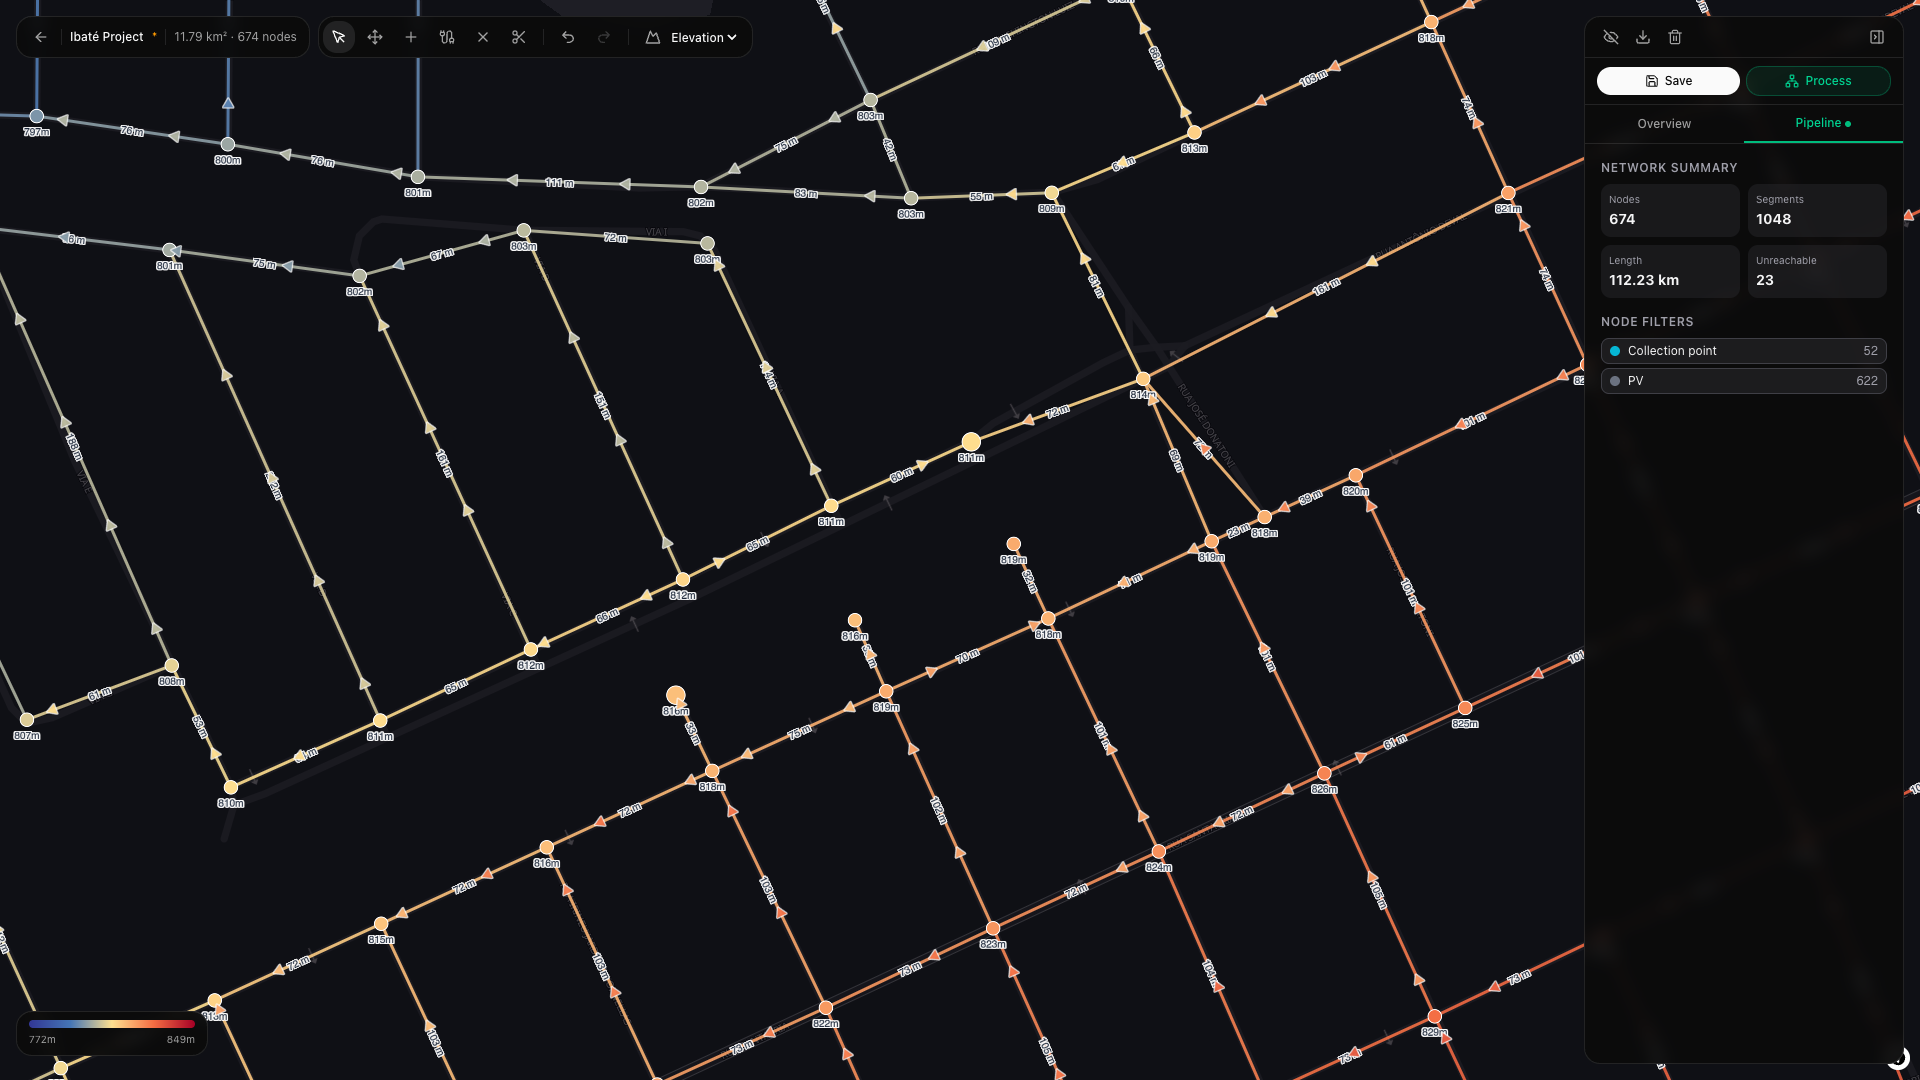
\includegraphics[width=\linewidth]{images/small-case-after-processing.png}
\end{minipage}
\caption{Local graph example before processing on the left and after sewer-network processing on the right.}
\label{fig:before-after-processing}
\end{figure}

The current validation is mainly functional and computational.
It verifies whether internal steps produce coherent structures: street extraction, elevation enrichment, graph construction, editing, persistence, routing, coverage preservation, and visualization of the processed network.
This validation already includes automated tests for geographic calculations, area validation, node rules, parity between implementations, classification, sanitization, extrema detection, edge cost, RSPH, coverage repair, cycle prevention, elevation handling, and node reduction.

Systematic experimental validation is still pending.
The planned stage considers applying the system to different urban areas in order to observe its behavior in street meshes and topographic conditions with distinct characteristics.
This stage should analyze aspects such as route coherence, manhole placement, collection point identification, street mesh coverage, redundant node reduction, gravitational direction, and generation time for the preliminary solution.

This distinction is important: automated tests increase confidence in internal parts of the system, but they do not replace real case studies or qualitative evaluation by a specialist.
Therefore, the prototype should be interpreted as a computational basis under development, suitable for preliminary conception and analysis, but still dependent on validation before any use as support for final engineering decisions.

\subsection{Building detection with machine learning}

Estimating sewage contribution in each segment of a collection network can depend on the type and density of the buildings served.
In traditional preliminary planning, this information may be collected manually or approximated by aggregated indicators, such as lot-frontage length \cite{rodrigues2020}.
For this reason, \method incorporates automatic building detection from satellite imagery as part of the research strategy for estimating sewage contribution with greater spatial granularity.
The goal of this component is to connect the physical layout of the sewer network with information about the built environment served by each segment, reducing dependence on coarse frontage-based approximations.

The study considers deep learning approaches for semantic segmentation, identifying the area occupied by buildings in medium- and high-resolution images.
Convolutional Neural Networks (CNNs) and Vision Transformers (ViTs) have shown strong performance in this task, extracting both local image patterns and long-range contextual relationships \cite{alidoost2018cnn,dosovitskiy2021imageworth16x16words}.
Recent hybrid architectures that combine CNNs and Transformers also indicate promising directions for dense urban scenarios \cite{zhang2024building,zhou2024hierarchical}.

Two pre-trained models were evaluated with fine-tuning on the Massachusetts Buildings Dataset \cite{MassachusettsBuildingsDataset}: SAM (\textit{Segment Anything Model}), a general segmentation model based on Transformers, and DeepLab V3, a CNN-based model with atrous convolutions.
Table~\ref{tab:seg_results} compares the segmentation results before and after fine-tuning.

\begin{table}[ht]
\centering
\caption{Building segmentation results before and after fine-tuning}
\label{tab:seg_results}
\begin{tabular}{lccc}
\hline
\textbf{Model} & \textbf{Fine-tuned} & \textbf{Mean IoU} & \textbf{Mean Dice} \\
\hline
SAM        & No  & 0.160 & --    \\
SAM        & Yes & 0.586 & 0.734 \\
DeepLab V3 & No  & 0.177 & 0.293 \\
DeepLab V3 & Yes & 0.600 & 0.747 \\
\hline
\end{tabular}
\end{table}

Fine-tuning produced expressive gains in both models.
SAM increased its mean IoU from 0.160 to 0.586, while DeepLab V3 increased from 0.177 to 0.600, with a mean Dice of 0.747.
These results indicate that building segmentation is a viable input for estimating sewage contribution in the \method workflow, especially when the platform must distinguish areas with different building densities inside the same selected region.

The next steps for this component include counting and classifying individual building instances by lot, investigating hybrid CNN-Transformer architectures, and exploring multimodal fusion with digital surface models for dense urban scenarios \cite{zhou2024hierarchical}.
